\documentclass{article}
\usepackage{graphicx}
\usepackage{amsmath}
\usepackage{url}

\title{Relatório — Lista 01}
\author{Vinicius Viroli Pereira}
\date{}

\begin{document}

\maketitle

\section{Variável escolhida}
A variável utilizada nesta atividade foi a \textbf{Temperatura}, presente no arquivo
\texttt{dados.csv}. Ela representa a temperatura média registrada em cada mês.

\section{Resumo estatístico}
O script \texttt{resumo.sh} calcula a média da variável utilizando a fórmula:



\[
\bar{x} = \frac{1}{n} \sum_{i=1}^{n} x_i
\]



Os resultados são salvos no arquivo \texttt{resumo.txt}, que contém os valores
calculados automaticamente a partir dos dados originais.

\section{Figura}
A seguir apresentamos a figura gerada pelo script \texttt{figura.R}:

\begin{figure}[h]
  \centering
  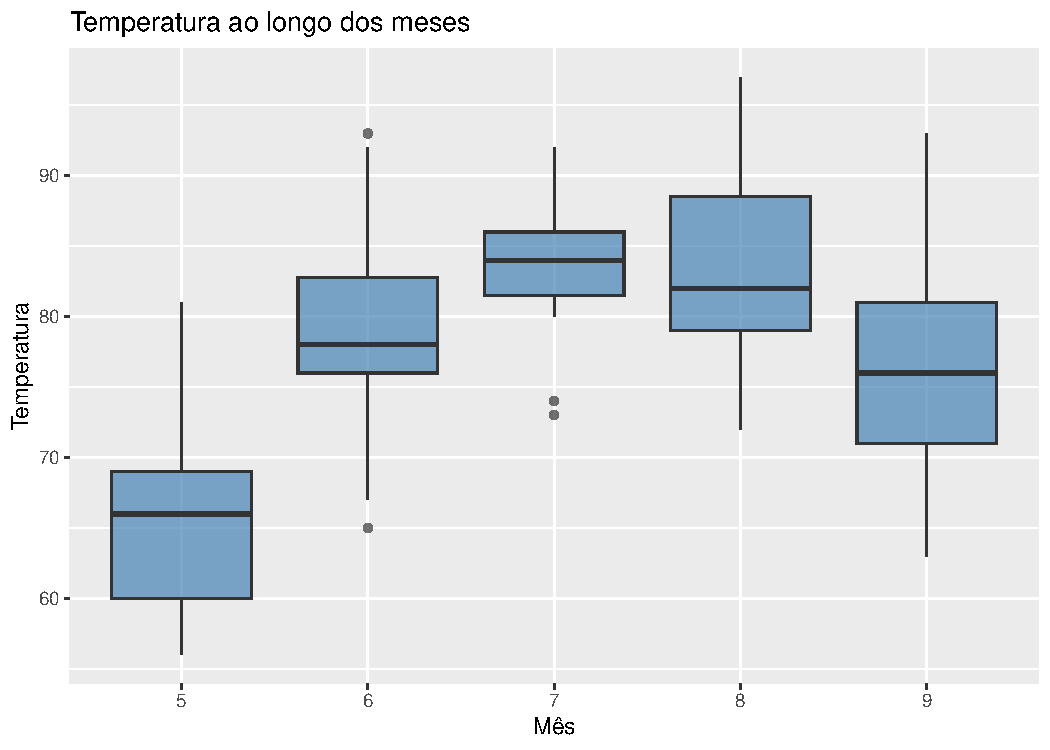
\includegraphics[width=0.8\textwidth]{figura.pdf}
  \caption{Temperatura ao longo dos meses}
  \label{fig:temperatura}
\end{figure}

A Figura~\ref{fig:temperatura} mostra a variação da temperatura ao longo dos meses.
É possível observar tendências, oscilações e possíveis padrões sazonais ao longo
do período analisado.

\section{Referências}
\begin{thebibliography}{9}

\bibitem{tdr}
Fernando Mayer,
\textit{Tecnologia de Dados},
\url{https://fernandomayer.github.io/tdr/}

\end{thebibliography}

\end{document}

